\subsubsection{Kesimpulan Pemilihan Alternatif}

\begin{figure}[ht]
	\centering
	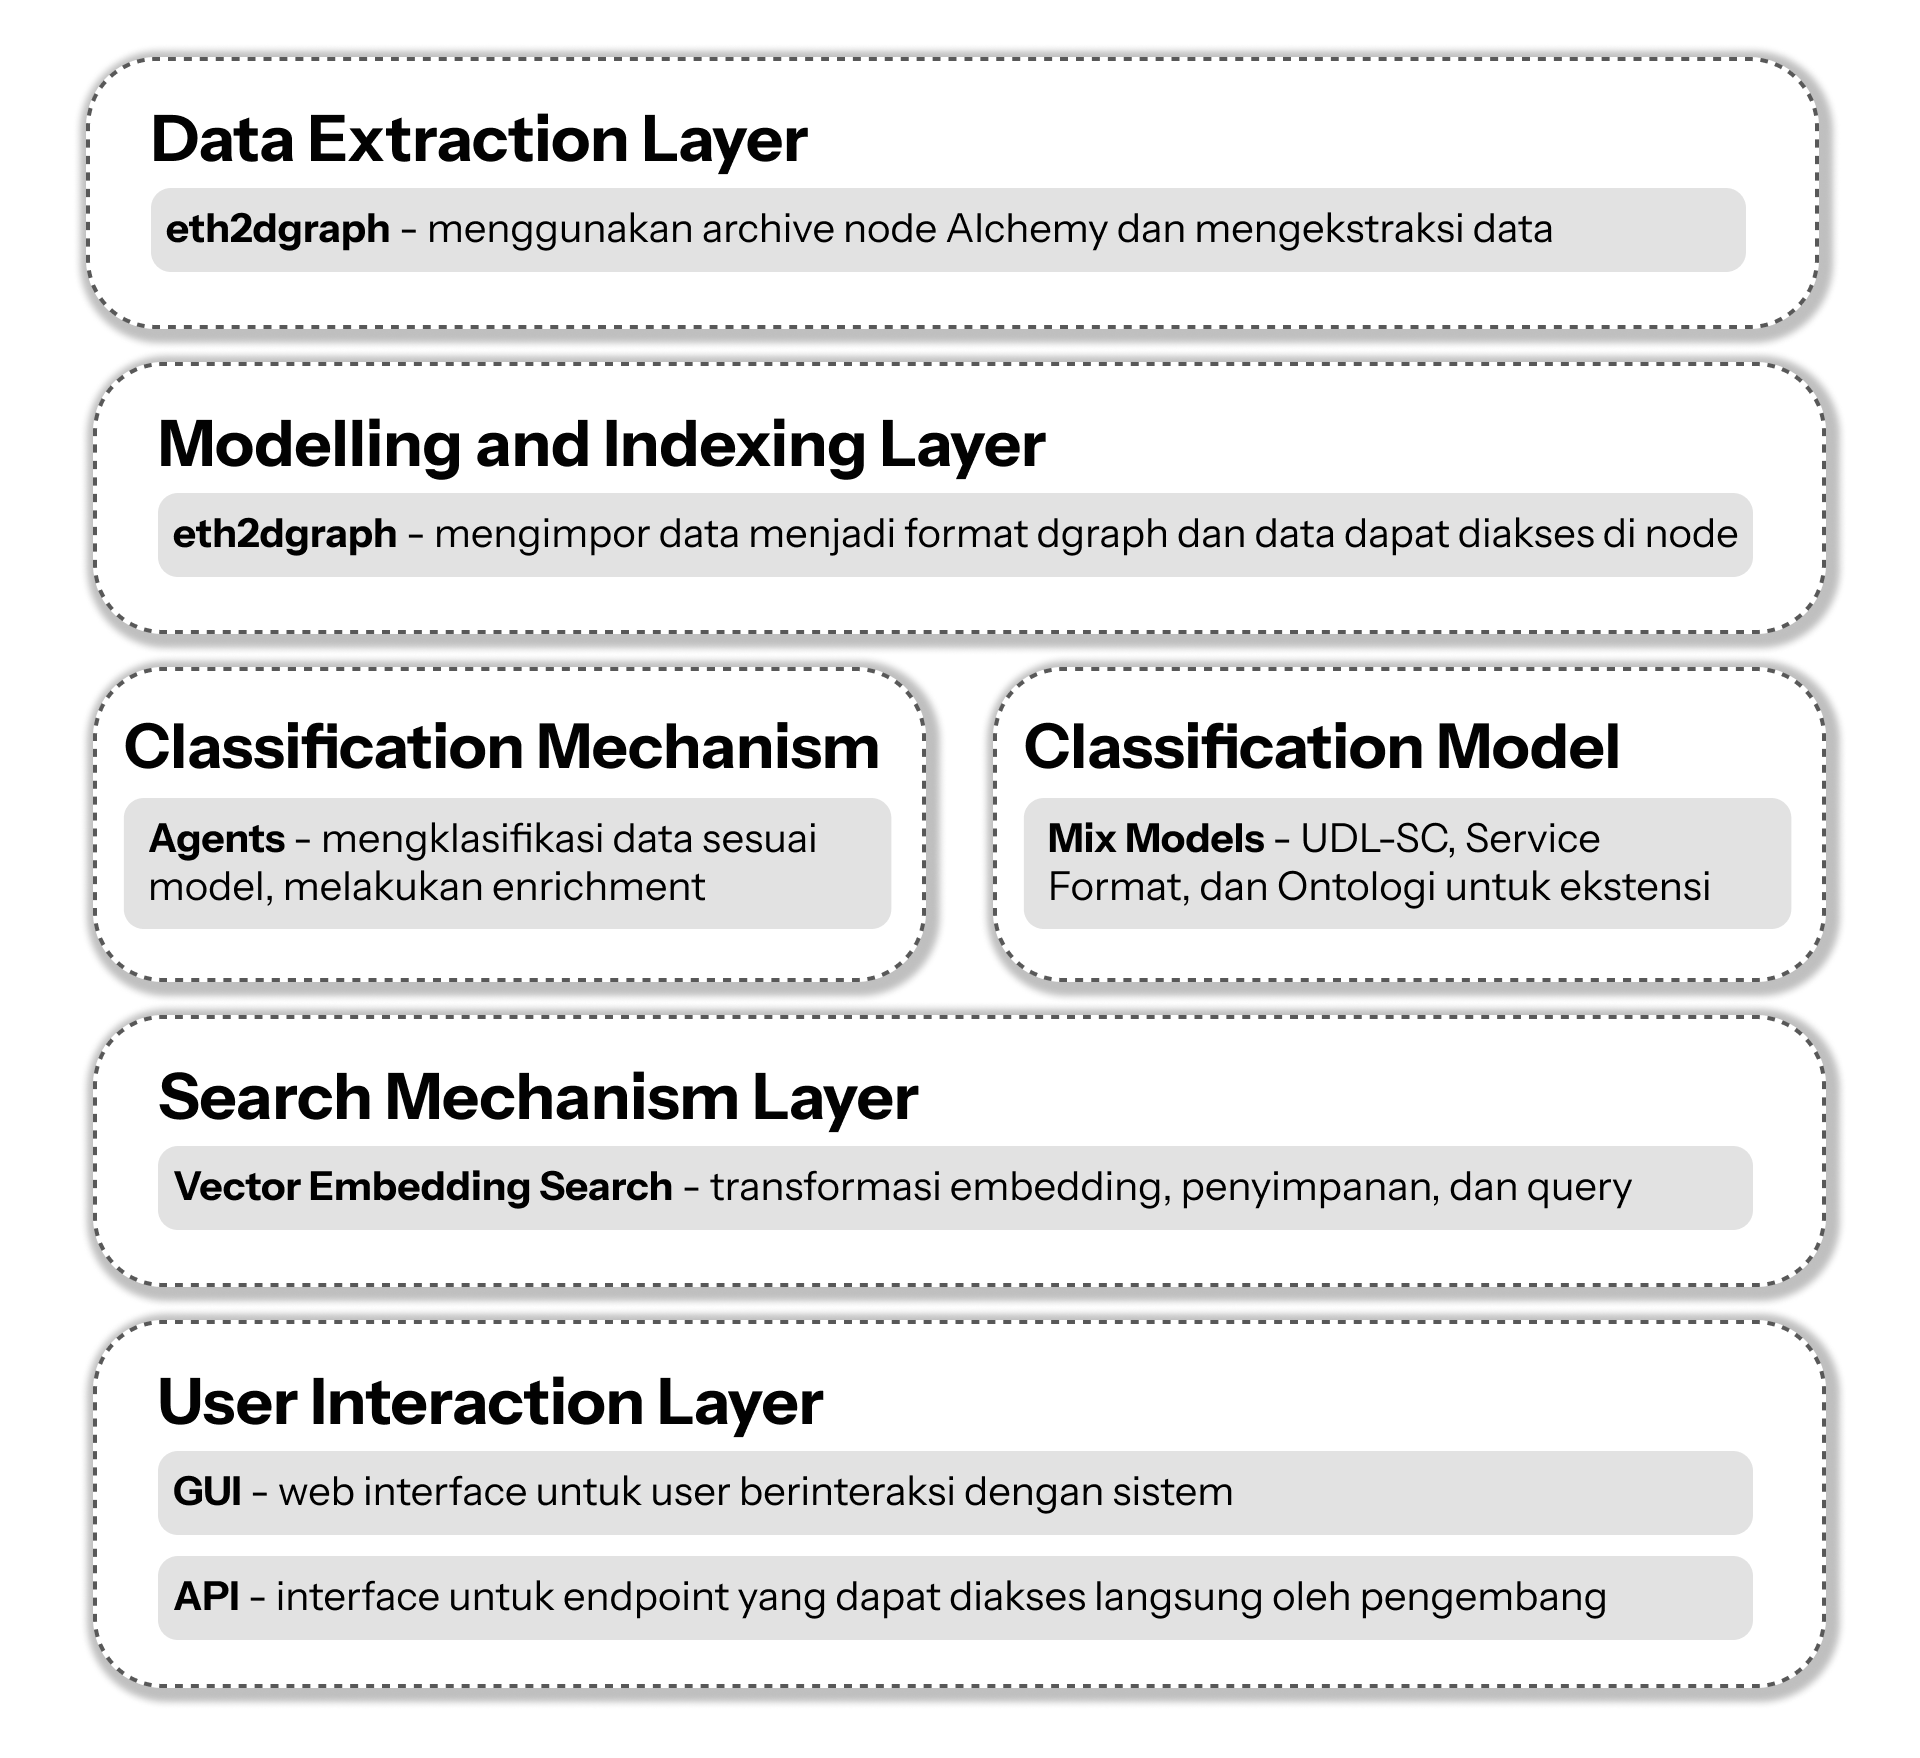
\includegraphics[width=0.7\textwidth]{resources/chapter-3/hasil-pemilihan.png}
	\caption{Kesimpulan pemilihan alternatif}
	\label{image:layer-architecture}
\end{figure}

Berdasarkan analisis dari alternatif-alternatif yang dibahas pada bagian \ref{subsec:analisis-alternatif-solusi}, dapat disimpulkan bahwa alternatif yang dipilih untuk membangun sistem adalah sebagai berikut:

\begin{enumerate}
	\item \textbf{Ekstraksi data Smart Contracts dari Blockchain Ethereum}: Alternatif yang dipilih adalah \textit{eth2dgraph} \parencite{aimar2023extraction}, karena memiliki aksesibilitas yang baik, bersifat \textit{open source}, memiliki kecepatan ekstraksi yang tinggi, dan juga menyediakan infrastruktur lengkap sampai pada penyimpanan data dalam format Distributed Graph Database.
	\item \textbf{Pemodelan, penyimpanan, dan \textit{indexing} data Smart Contracts}: Alternatif yang dipilih adalah \textit{eth2dgraph} \parencite{aimar2023extraction}, karena memiliki kemampuan skalabilitas tinggi dan dapat melakukan query dengan efisien. Selain itu, Dgraph juga memiliki kemampuan untuk melakukan \textit{indexing} data dengan baik.
	\item \textbf{Klasifikasi fungsional dan semantik Smart Contracts}: Alternatif yang dipilih untuk mekanisme klasifikasi adalah LLM Classification, karena memliki kemampuan kustomisasi yang baik untuk mendeskripsikan dan mengklasifikasi Smart Contracts. Model yang akan digunakan adalah model tekstual, yaitu penjelasan fungsionalitas Smart Contracts dalam bahasa alami, dengan kombinasi dengan konsep ontologi dalam bentuk metadata untuk pengklasifikasian. Metadata dengan konsep ontologi ini akan membuat atribut data lebih mudah untuk diekstrak menjadi sebuah ontologi.
	\item \textbf{Pencarian dan rekomendasi Smart Contracts}: Alternatif yang dipilih untuk mekanisme pencarian awal adalah alternatif Vector Embedding Search, karena simplisitas yang ditawarkan dan tidak ada redundansi \textit{layer}. Alternatif yang dapat dikonsiderasikan untuk pengembangan berikutnya, terutama jika dikembangkan sebuah fitur untuk berinteraksi dengan sistem yang lebih kompleks adalah alternatif \textit{Retrieval-Augmented Generation (RAG)}, karena dapat mengakomodasi interaksi yang lebih kompleks.
	\item \textbf{Interaksi pengguna dengan sistem}: API dan GUI akan diimplementasikan untuk interaksi pengguna dengan sistem karena dapat memberikan fleksibilitas dan kemudahan bagi pengguna. Sehingga, pengguna dapat melakukan pencarian Smart Contracts dengan cara yang sesuai dengan kebutuhan mereka.
\end{enumerate}